\chapter{Números Inteiros}

\begin{list}{\textbf{Questão \arabic{quest}.}}{\usecounter{quest}}
%define a margem da lista.	
%\setlength{\labelwidth}{-2mm} \setlength{\parsep}{0mm}
%\setlength{\topsep}{0mm} \setlength{\leftmargin}{-2mm}
\renewcommand{\labelenumi}{(\alph{enumi})}

\item Registre usando números positivos, negativos ou zero.
		\begin{enumerate}
			\item uma altitude de 50 m acima do nível do mar.
			\item a altitude de  43 m abaixo do nível do mar.
			\item a altitude ao nível do mar.
		\end{enumerate}
		
		\item Em uma cidade de Europa, foi registrada a temperatura ao meio-dia durante os oito primeiros dias de janeiro de certo ano. Veja  resultado das anotações no gráfico abaixo, que relaciona cada dia à temperatura correspondente.
		
		\begin{center}
				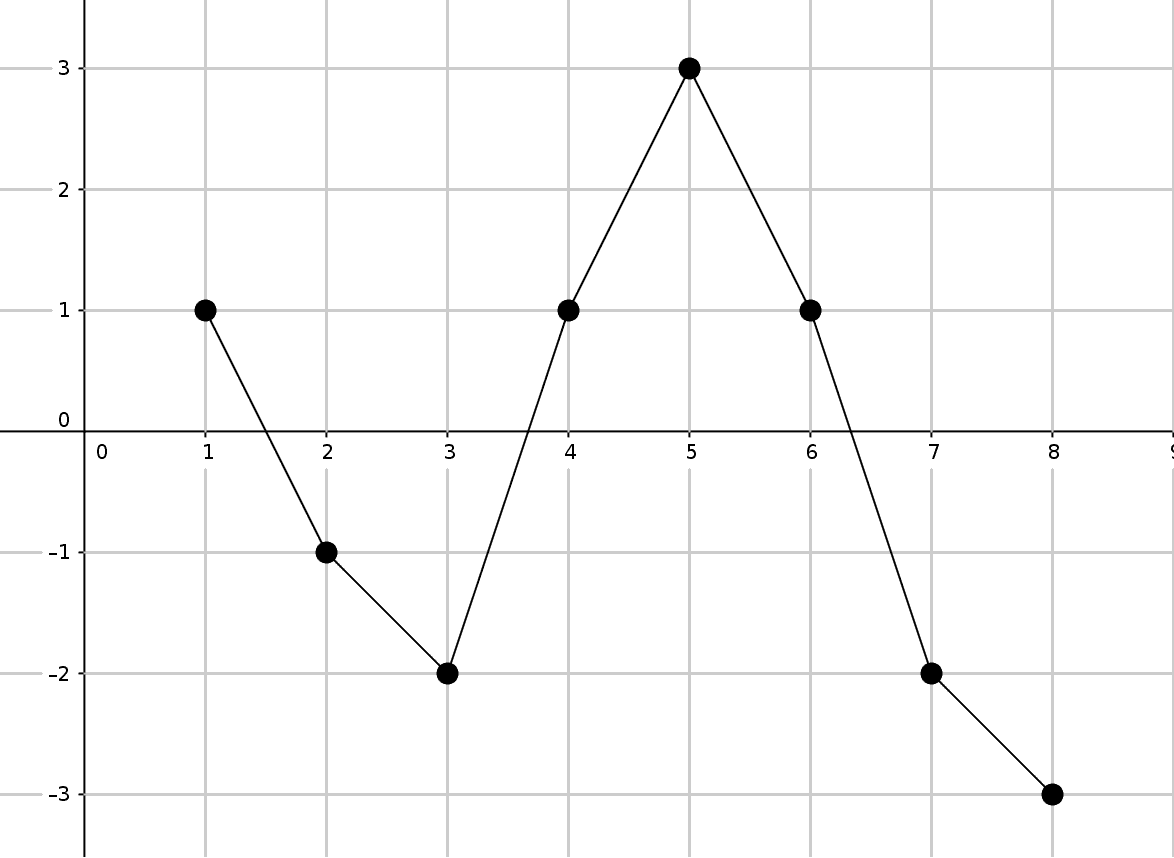
\includegraphics[scale=0.25]{figuras/fig42.png}.
		\end{center}		
		\begin{enumerate}
			\item Qual foi a temperatura máxima registrada nesses dias? Em que dia ocorreu?
			\item Qual foi temperatura mínima? Em que dia ocorreu?
			\item Em que dia a temperatura registrada foi de 0º C?
			\item Qual foi a temperatura registrada no dia 2?
		\end{enumerate}
		
		\item Localize na reta os pontos dados.
		\begin{center}
			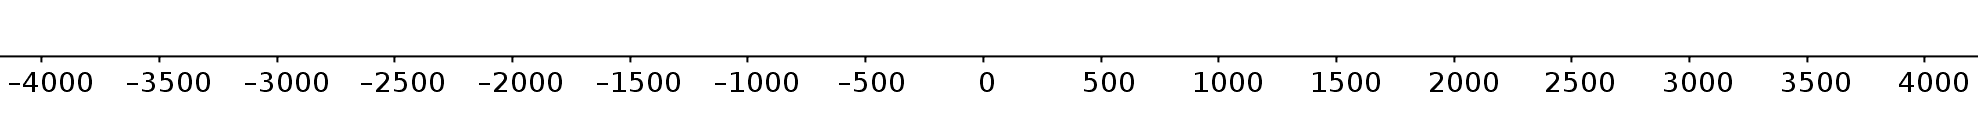
\includegraphics[scale=0.33]{figuras/fig43.png}
		\end{center}
		Coloque na reta os seguintes pontos.
		\begin{multicols}{5}
		\begin{enumerate}
			\item 476
			\item -753
			\item 391
			\item -540
			\item -405
		\end{enumerate}
		\end{multicols}
		\item Responda:
		\begin{enumerate}
			\item Em que ano morreu uma pessoa que nasceu no ano -15 e viveu 60 anos?
			\item Quantos anos viveu uma pessoa que nasceu no ano -75 e morreu no ano +5?
			\item Em que ano nasceu uma pessoa que viveu 92 anos e morreu no ano -20?
		\end{enumerate}
		
		\item Efetue a subtração correspondente a cada situação e escreva qual a temperatura resultante.		
		\begin{enumerate}
			\item A temperatura era de 18º C e baixou 4ºC.
			\item A temperatura era de 10ºC e baixou 10ºC.
			\item A temperatura era de 2ºC e baixou 5ºC.
			\item A temperatura era de 0ºC e baixou 7ºC.
		\end{enumerate}
		
		\item Considere o conjunto dos números inteiros e escreva:
		\begin{multicols}{2}		
		\begin{enumerate}
			\item o sucessor de 8.
			\item o antecessor de 0.
			\item o sucessor de 50.
			\item o sucessor de -2.
			\item o antecessor de -2.
			\item o antecessor de -69.
		\end{enumerate}
		\end{multicols}
		
		\item Coloque entre cada $\square$ o símbolo de pertence $(\in)$ ou de não pertence $(\notin)$.
		\begin{multicols}{3}
		\begin{enumerate}
			\item -6 $\square\ \mathbb{N}$ 
			\item -2 $\square\ \mathbb{Z}$ 
			\item -0 $\square\ \mathbb{Z}$
			\item 16 $\square\ \mathbb{N}$
			\item +13 $\square\ \mathbb{Z}$   
			\item 2,7 $\square\ \mathbb{Z}$ 
		\end{enumerate}		
		\end{multicols}
		
		\item Escreva:
		\begin{multicols}{2}
		\begin{enumerate}
			\item um número inteiro que não é natural.
			\item um número natural que não é inteiro.
		\end{enumerate}
		\end{multicols}
		
		\item Observe a reta numerada, a seguir, e escreva a localização dos seguintes pontos em relação à origem.
		\newline
		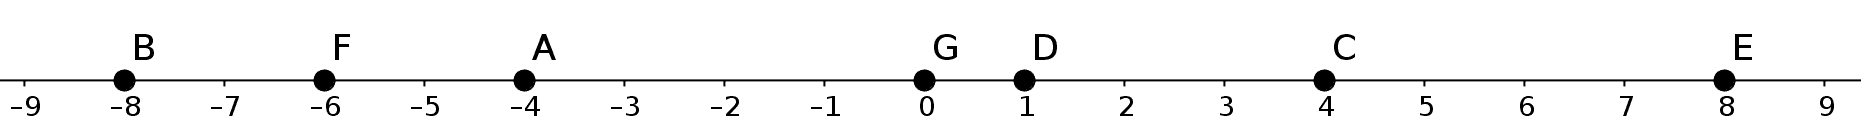
\includegraphics[scale=0.3]{figuras/fig44.png} 		
		\begin{multicols}{3}
		\begin{enumerate}
			\item A = 
			\item B = 
			\item C =
			\item D =
			\item E =
			\item F = 
		\end{enumerate}
		\end{multicols}
		
		\item Determine:
		\begin{multicols}{3}
		\begin{enumerate}
			\item |-2| 
			\item |150|
			\item |-7|
			\item |-50|
			\item |-3| + 3 + |-5|
			\item |5| + |4| + |-5|
		\end{enumerate}
		\end{multicols}
		
		\item Determine o oposto ou simétrico  de cada número.
		\begin{multicols}{3}
		\begin{enumerate}
			\item -7 
			\item 200
			\item -53
			\item 55
			\item 1 000
			\item -5 000
		\end{enumerate}
		\end{multicols}
		
		\item Complete com >, < ou = os espaços entre os números. Use o processo que julgar mais conveniente.
		\begin{multicols}{4}
		\begin{enumerate}
			\item 86 \ \ -100
			\item 623 \ \ 519
			\item -374 \ \ -200
			\item 0 \ \ -6
			\item 0 \ \ 11
			\item +8 \ \ 8
			\item +4 \ \ -4
			\item -6 \ \ +2
			\item +6 \ \ -2
			\item -18 \ \ 0
			\item +16 \ \ 0
			\item -3 \ \ +9
		\end{enumerate}
		\end{multicols}
		
		\item Efetue as adições.
		\begin{multicols}{3}
		\begin{enumerate}
			\item $-2-2$
			\item $(-3)+(+3)$
			\item $+2-0$
			\item $(-3)+(+3)$
			\item $+2-0$
			\item $+4-6$
			\item $(-5)+(+7)$
			\item $(-3)+(-4)$
			\item $(+3) +0$
			\item $+6+1$
			\item $+5-4$
			\item $(-12)+(-15)$
			\item $ +23+30$
			\item $(+17)+(+49)$
			\item $-132-29$
			\item $(+51)+(-51)$
			\item $-80+30$
			\item $-27+30$
			\item $(+230)+(-201)$
			\item $-37+37$
			\item $+46-59$
		\end{enumerate}
		\end{multicols}
		
		\item Escreva e efetue a adição correspondente a cada situação e indique o novo saldo.
		\begin{enumerate}
			\item O saldo de José era negativo de R\$ 150,00 e ele fez um depósito de R\$ 200,00.
			\item O saldo de Ana era positivo de R\$ 95,00, e ela realizou uma retirada de R\$ 150,00.
			\item O saldo de Sílvio era negativo de R\$ 55,00, e ele efetuou uma retirada de R\$ 60,00.
			\item O saldo de Sueli era zero, e ela fez um depósito de R\$ 300,00.
			\item O saldo de Sérgio era positivo de R\$ 427,00, e ele realizou um depósito de R\$ 248,00.
		\end{enumerate}
		
		\item Use o processo que julgar mais conveniente, como estudado nas aulas, e calcule:
		\begin{multicols}{2}
		\begin{enumerate}
			\item $-12+4+11-8+13 +1$
			\item $(+6)+(-14)+(-7)+(6)+(+9)$
			\item $-2+5+3-2+1$
			\item $-7-3-9+8-1-4$
			\item $(+16)+(-29)+(+33)+(-37)$
			\item $(-3)+(-5)+(-2)+(-1)$
		\end{enumerate}
		\end{multicols}
		
		\item Vamos imaginar o movimento de um elevador em um prédio de 8 andares (acima do térreo) e 3 subsolos, como indica a figura ao lado. Complete a tabela abaixo. Na última coluna, indique a operação efetuada (adição ou subtração.)
		\newline
		\newline
		\begin{tabular}{|c|c|c|c|}
		\hline 
		Andar da saída & Deslocamento do elevador & Andar de chegada & Operação efetuada \\ 
		\hline 
		-1 & +3 &   &   \\ 
		\hline 
		-2 & -1 &   &   \\ 
		\hline 
		+3 &   & -3 &   \\ 
		\hline 
		  & +2 & +2 &   \\ 
		\hline 
		0 & -2 &   &   \\ 
		\hline 
		-3 &   & -1 &   \\ 
		\hline 
		\end{tabular} 
		
		\item Efetue estas multiplicações que envolvem todos os casos estudados.
		\begin{multicols}{3}
		\begin{enumerate}
			\item $(-7)\cdot(-11)$
			\item $(+4)\cdot(+3)$
			\item $(-14)\cdot0$
			\item $(-8)\cdot(+9)$
			\item $0\cdot(-342)$
			\item $(+12)\cdot(-12)$
		\end{enumerate}
		\end{multicols}
		
		\item Calcule:
		\begin{multicols}{4}
		\begin{enumerate}
			\item $(2)^5$
			\item $(+10)^{10}$
			\item $(-3)^4$
			\item $(-2)^5$
			\item $(+1)^3$
			\item $(+1)^2$
			\item $(-1)^5$
			\item $(-1)^4$
		\end{enumerate}
		\end{multicols}
\end{list}